\documentclass[xetex,mathserif,serif]{beamer}

\usepackage{xunicode}
\usepackage{xltxtra}
\usepackage{color}
\usepackage{url}
\usepackage{listings}
\usepackage{fontspec}
\usepackage{geometry}
\usepackage{lastpage}
\usepackage{fancyhdr}
\usepackage{amsmath}
\usepackage{amsthm}
\usepackage{amssymb}
\usepackage{blkarray}
\usepackage{multicol}
\usepackage{relsize}

\definecolor{solarized@base03}{HTML}{002B36}
\definecolor{solarized@base02}{HTML}{073642}
\definecolor{solarized@base01}{HTML}{586e75}
\definecolor{solarized@base00}{HTML}{657b83}
\definecolor{solarized@base0}{HTML}{839496}
\definecolor{solarized@base1}{HTML}{93a1a1}
\definecolor{solarized@base2}{HTML}{EEE8D5}
\definecolor{solarized@base3}{HTML}{FDF6E3}
\definecolor{solarized@yellow}{HTML}{B58900}
\definecolor{solarized@orange}{HTML}{CB4B16}
\definecolor{solarized@red}{HTML}{DC322F}
\definecolor{solarized@magenta}{HTML}{D33682}
\definecolor{solarized@violet}{HTML}{6C71C4}
\definecolor{solarized@blue}{HTML}{268BD2}
\definecolor{solarized@cyan}{HTML}{2AA198}
\definecolor{solarized@green}{HTML}{859900}
\definecolor{yaleblue}{HTML}{0E4C92}

\setbeamertemplate{navigation symbols}{}
% \setbeamerfont{title}{family=\old}
% \setbeamerfont{author}{family=\tfont}%
% \setbeamerfont{frametitle}{family=\oldA}
% \setbeamerfont{date}{family=\dfont}

\setbeamertemplate{itemize items}{--}
\setbeamercolor*{item}{fg=black}

\defaultfontfeatures{Mapping=tex-text}
\hypersetup{pdfstartview={FitH}}

\newcommand{\old}[1]{\fontspec[Alternate=1,Ligatures={Common}]{Hoefler Text}\fontsize{18pt}{30pt}\selectfont #1}%
\newcommand{\oldA}[1]{\fontspec[Alternate=1,Ligatures={Common, Rare}]{Hoefler Text}\fontsize{12pt}{15pt}\selectfont #1}%
\newcommand{\oldB}[1]{\fontspec[Ligatures={Common}]{Didot}\fontsize{12pt}{15pt}\color{solarized@base02}\selectfont #1}%
\newcommand{\tfont}[1]{\fontspec[Alternate=1,Ligatures={Common}]{Hoefler Text}\fontsize{12pt}{20pt}\selectfont #1}%
\newcommand{\dfont}[1]{\fontspec[Ligatures={Common}]{Didot}\fontsize{12pt}{12pt}\selectfont #1}%

\newcommand{\minimize}{\mathop{\mathrm{minimize}}}
\newcommand{\argmin}{\mathop{\mathrm{arg\,min}}}
\newcommand{\argmax}{\mathop{\mathrm{arg\,max}}}
\newcommand{\st}{\mathop{\mathrm{subject\,\,to}}}

\newcommand\independent{\protect\mathpalette{\protect\independenT}{\perp}}
\def\independenT#1#2{\mathrel{\rlap{$#1#2$}\mkern2mu{#1#2}}}

\setlength{\parindent}{0pt}
\setlength{\parskip}{12pt}

\setromanfont [Ligatures={Common}, Numbers={OldStyle}, Variant=01,
 BoldFont={LinLibertine_RB.otf},
 ItalicFont={LinLibertine_RI.otf},
 BoldItalicFont={LinLibertine_RBI.otf}
 ]{LinLibertine_R.otf}



\title{high performance data i/o}
\date{2015-02-16}

\begin{document}

%%%%%%%%%%%%%%%%%%%%%%%%%%%%%%%%%%%%%%%%%%%%%%%%%%%
\begin{frame}[fragile] \frametitle{}

\vfill

{\fontsize{0.7cm}{0cm}\selectfont Lecture 02 \\\vspace{0.2cm} Simple Linear Models: OLS}\\\vspace{0.5cm}
04 September 2015

\vspace{2cm}

\begin{minipage}{0.6\textwidth}
Taylor B. Arnold \\
Yale Statistics \\
STAT 312/612
\end{minipage}
\hfill
\begin{minipage}{0.3\textwidth}\raggedleft

\includegraphics[scale=0.3]{../yale-logo.png}
\end{minipage}%

\end{frame}

%%%%%%%%%%%%%%%%%%%%%%%%%%%%%%%%%%%%%%%%%%%%%%%%%%%
\begin{frame}[fragile] \frametitle{}

\begin{flushright}
{\color{yaleblue}\sc\fontsize{1cm}{0cm}\selectfont Office Hours}
\end{flushright}

\end{frame}


%%%%%%%%%%%%%%%%%%%%%%%%%%%%%%%%%%%%%%%%%%%%%%%%%%%
\begin{frame}[fragile] \frametitle{}

\begin{itemize}
\item Taylor Arnold:
\begin{itemize}
\item 24 Hillhouse, Office \# 206
\item Wednesdays 13:30-15:00, or by appointment
\item Short one-on-one meetings (or small groups)
\end{itemize}
\item Jason Klusowski:
\begin{itemize}
\item 24 Hillhouse, Main Classroom
\item Tuesdays 19:00-20:30
\item Group Q\&A style
\end{itemize}
\end{itemize}

\end{frame}

%%%%%%%%%%%%%%%%%%%%%%%%%%%%%%%%%%%%%%%%%%%%%%%%%%%
\begin{frame}[fragile] \frametitle{}

\begin{flushright}
{\color{yaleblue}\sc\fontsize{1cm}{0cm}\selectfont Website}
\end{flushright}

\end{frame}


%%%%%%%%%%%%%%%%%%%%%%%%%%%%%%%%%%%%%%%%%%%%%%%%%%%
\begin{frame}[fragile] \frametitle{}

{\fontsize{0.5cm}{0cm}\selectfont
\url{http://euler.stat.yale.edu/~tba3/stat612}
}

\end{frame}

%%%%%%%%%%%%%%%%%%%%%%%%%%%%%%%%%%%%%%%%%%%%%%%%%%%
\begin{frame}[fragile] \frametitle{}

{\color{yaleblue}\fontsize{16pt}{20pt}\selectfont Goals for today}

\begin{enumerate}
\item calculate the MLE for simple linear regression
\item derive basic properties of the simple linear model MLE
\item introduction to R for simulations and data analysis
\end{enumerate}

\end{frame}

%%%%%%%%%%%%%%%%%%%%%%%%%%%%%%%%%%%%%%%%%%%%%%%%%%%
\begin{frame}[fragile] \frametitle{}

\begin{flushright}
{\color{yaleblue}\sc\fontsize{1cm}{0cm}\selectfont Simple Linear Models:\\\vspace{0.2cm} MLEs}
\end{flushright}

\end{frame}

%%%%%%%%%%%%%%%%%%%%%%%%%%%%%%%%%%%%%%%%%%%%%%%%%%%
\begin{frame}[fragile] \frametitle{}

Considering observing $n$ samples
from a simple linear model with only a single unknown
slope parameter $\beta \in \mathbb{R}$, \pause
\begin{align*}
y_i &= x_i\beta  + \epsilon_i, \quad i = 1, \ldots n.
\end{align*}
This is, perhaps, the simpliest linear model.

\end{frame}

%%%%%%%%%%%%%%%%%%%%%%%%%%%%%%%%%%%%%%%%%%%%%%%%%%%
\begin{frame}[fragile] \frametitle{}

For today, we will assume that the $x_i$'s are fixed and
known quantities. This is called a {\bf fixed design}, compared
to a {\bf random design}.

\end{frame}

%%%%%%%%%%%%%%%%%%%%%%%%%%%%%%%%%%%%%%%%%%%%%%%%%%%
\begin{frame}[fragile] \frametitle{}

The error terms are assumed to be independent and identically
distributed random variables with a normal density function:
\begin{align*}
\epsilon_i \sim \mathcal{N}(0, \sigma^2)
\end{align*}
For some unknown variance $\sigma^2 > 0$.

\end{frame}

%%%%%%%%%%%%%%%%%%%%%%%%%%%%%%%%%%%%%%%%%%%%%%%%%%%
\begin{frame}[fragile] \frametitle{}

\begin{center}
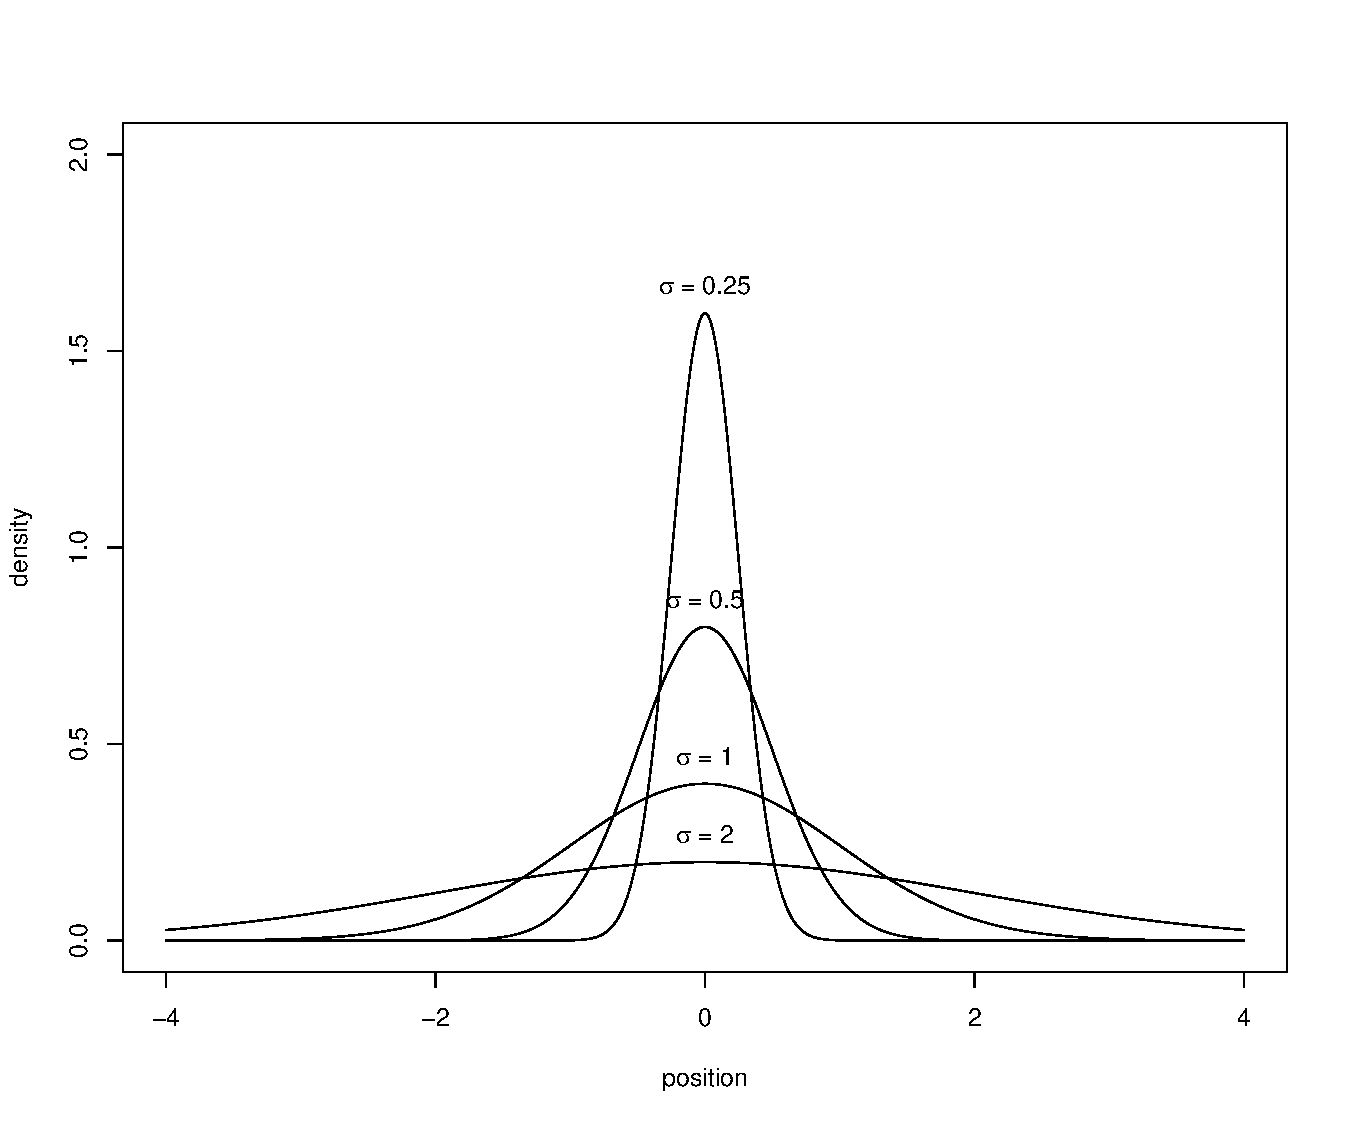
\includegraphics[width=\linewidth]{img/normal_density.pdf}
\end{center}

\end{frame}

%%%%%%%%%%%%%%%%%%%%%%%%%%%%%%%%%%%%%%%%%%%%%%%%%%%
\begin{frame}[fragile] \frametitle{}

The density function of a normally distributed random variable with
mean $\mu$ and variance $\sigma^2$ is given by:
\begin{align*}
f(x) &=  \frac{1}{\sqrt{2\pi\sigma^2}} \times
    exp \left\{ - \frac{1}{2\sigma^2} (x-\mu)^2 \right\}
\end{align*}
\pause Conceptually, the front term is just a normalization to make
the density sum to $1$. The important part is:
\begin{align*}
f(x) &\propto exp \left\{ - \frac{1}{2\sigma^2} (x-\mu)^2 \right\}
\end{align*}

\end{frame}

%%%%%%%%%%%%%%%%%%%%%%%%%%%%%%%%%%%%%%%%%%%%%%%%%%%
\begin{frame}[fragile] \frametitle{}

Which you have probably seen rewritten as:
\begin{align*}
f(x) &\propto exp \left\{ - 0.5 \cdot \left(\frac{x-\mu}{\sigma}\right)^2 \right\}
\end{align*}

\end{frame}

%%%%%%%%%%%%%%%%%%%%%%%%%%%%%%%%%%%%%%%%%%%%%%%%%%%
\begin{frame}[fragile] \frametitle{}

Let's look at the maximum likelihood function of this model:
\begin{eqnarray*}
\mathcal{L} (\beta, \sigma | x, y) &=& \prod_i \mathcal{L} (\beta, \sigma | x_i, y_i) \\ \pause
&=& \prod_i \frac{1}{\sqrt{2\pi\sigma^2}} \times
    exp \left\{ - \frac{1}{2\sigma^2} {\color{solarized@red} (y_i - \beta x_i)^2} \right\}
\end{eqnarray*}
\pause Notice that the {\color{solarized@red}mean $\mu$} from the general case has been
replaced by $\beta x_i$, which should be the mean of $y_i | x_i$.

\end{frame}

%%%%%%%%%%%%%%%%%%%%%%%%%%%%%%%%%%%%%%%%%%%%%%%%%%%
\begin{frame}[fragile] \frametitle{}

We can bring the product up into the the exponent as a sum:
\begin{eqnarray*}
\mathcal{L} (\beta, \sigma | x, y) &=& {\color{solarized@blue}\prod_i} \frac{1}{\sqrt{2\pi\sigma^2}} \times
    exp \left\{ - \frac{1}{2\sigma^2} (y_i - \beta x_i)^2 \right\} \\ \pause
&=& (2\pi\sigma^2)^{-{\color{solarized@blue}n}/2} \times
    exp \left\{ - \frac{1}{2\sigma^2} \cdot {\color{solarized@blue}\sum_i} (y_i - \beta x_i)^2 \right\} \\
\end{eqnarray*}

\end{frame}

%%%%%%%%%%%%%%%%%%%%%%%%%%%%%%%%%%%%%%%%%%%%%%%%%%%
\begin{frame}[fragile] \frametitle{}

Let's highlight the slope parameter $\beta$:
\begin{eqnarray*}
\mathcal{L} (\beta, \sigma | x, y) &=& (2\pi\sigma^2)^{-n/2} \times
    exp \left\{ - \frac{1}{2\sigma^2} \cdot \sum_i (y_i -  {\color{solarized@orange} \bf \beta} x_i)^2 \right\} \\
\end{eqnarray*}
\pause What is the MLE for ${\color{solarized@orange} \bf \beta}$?

\end{frame}

%%%%%%%%%%%%%%%%%%%%%%%%%%%%%%%%%%%%%%%%%%%%%%%%%%%
\begin{frame}[fragile] \frametitle{}

Without resorting to any fancy math, we can see that:
\begin{align}
\widehat{\beta}_{MLE} &= \argmin_{b \in \mathbb{R}} \left\{ \sum_i (y_i -  b \cdot x_i)^2 \right\}
\end{align}
The least squares estimator.

\end{frame}

%%%%%%%%%%%%%%%%%%%%%%%%%%%%%%%%%%%%%%%%%%%%%%%%%%%
\begin{frame}[fragile] \frametitle{}

A slightly more `mathy' approach would be to calculate the the negative log-likelihood: \pause
\begin{align*}
-\text{log} \left\{ \mathcal{L} (\beta, \sigma | x, y)\right\} &= \frac{n}{2} \cdot \text{log}(2\pi\sigma^2) +
    \frac{1}{2\sigma^2}  \sum_i (y_i - \beta x_i)^2
\end{align*}
\pause Now the minimum of this corrisponds with the maximum likelihood estimators.

\end{frame}

%%%%%%%%%%%%%%%%%%%%%%%%%%%%%%%%%%%%%%%%%%%%%%%%%%%
\begin{frame}[fragile] \frametitle{}

Again, we notice that only the second term depends on $\beta$: \pause
\begin{align*}
-\text{log} \left\{ \mathcal{L} (\beta, \sigma | x, y)\right\} &= \frac{n}{2} \cdot \text{log}(2\pi\sigma^2) +
    {\color{solarized@orange} \frac{1}{2\sigma^2}  \sum_i (y_i - \beta x_i)^2}
\end{align*}
\pause And we can again see without resorting
to derivatives that the maximum likelihood estimator is that one that
minimizes the sum of squares:
\begin{align*}
\widehat{\beta}_{mle} = \argmin_{b \in \mathbb{R}} \left\{ \sum_i (y_i - b x_i)^2 \right\}
\end{align*}

\end{frame}

%%%%%%%%%%%%%%%%%%%%%%%%%%%%%%%%%%%%%%%%%%%%%%%%%%%
\begin{frame}[fragile] \frametitle{}

It is possible to directly solve the least squares and obtain
an analytic solution to the simple linear regression model.

Taking the derivative of the sum of squares with respect to
$\beta$ we get:
\begin{eqnarray*}
\frac{\partial}{\partial \beta} \sum_i (y_i - \beta x_i)^2
  &= 2 \cdot \sum_i ( y_i - \beta x_i) \cdot x_i \\ \pause
  &= 2 \cdot \sum_i ( y_i x_i - \beta x_i^2)
\end{eqnarray*}


\end{frame}

%%%%%%%%%%%%%%%%%%%%%%%%%%%%%%%%%%%%%%%%%%%%%%%%%%%
\begin{frame}[fragile] \frametitle{}

Setting the derivative equal to zero:
\begin{eqnarray*}
2 \cdot \sum_i ( y_i x_i - \widehat{\beta} x_i^2) &=& 0 \\ \pause
\sum_i y_i x_i &=& \widehat{\beta} \sum_i x_i^2 \\ \pause
\widehat{\beta}_{MLE} &=& \frac{\sum_i y_i x_i}{\sum_i x_i^2}
\end{eqnarray*}
\pause If you have seen the standard simple least squares solution
(that is, with an intercept) this should look familiar.

\end{frame}


%%%%%%%%%%%%%%%%%%%%%%%%%%%%%%%%%%%%%%%%%%%%%%%%%%%
\begin{frame}[fragile] \frametitle{}

There are many ways of thinking about the maximum likelihood estimator,
one of which is as a weighted sum of the data points $y_i$:
\begin{align*}
\widehat{\beta} &= \frac{\sum_i y_i x_i}{\sum_i x_i^2} \\
&= \sum_i \left( y_i \cdot \frac{x_i}{\sum_j x_i^2} \right) \\
&= \sum_i y_i w_i
\end{align*}

\end{frame}

%%%%%%%%%%%%%%%%%%%%%%%%%%%%%%%%%%%%%%%%%%%%%%%%%%%
\begin{frame}[fragile] \frametitle{}

One thing that the weighted form of the estimator makes
obvious is that the estimator is distributed normally:
\begin{align*}
\widehat{\beta} \sim \mathcal{N} (\cdot, \cdot)
\end{align*}
As it is the sum of normally distributed variables ($y_i$).

\end{frame}

%%%%%%%%%%%%%%%%%%%%%%%%%%%%%%%%%%%%%%%%%%%%%%%%%%%
\begin{frame}[fragile] \frametitle{}

The mean of the estimator becomes
\begin{eqnarray*}
\mathbb{E} \widehat{\beta} &=& \sum_i \mathbb{E} (y_i w_i) \\ \pause
&=& \sum_i w_i \cdot \mathbb{E} (y_i) \\ \pause
&=& \sum_i \beta x_i w_i \\ \pause
&=& \beta \cdot \sum_i x_i \frac{x_i}{\sum_j x_j^2} \\
&=& \pause \beta
\end{eqnarray*}
And so we see the estimator is unbiased.

\end{frame}

%%%%%%%%%%%%%%%%%%%%%%%%%%%%%%%%%%%%%%%%%%%%%%%%%%%
\begin{frame}[fragile] \frametitle{}

A normally distributed random variable is entirely characterised
by its mean and variance. So let us compute the variance of our
MLE estimator:
\begin{eqnarray*}
\mathbb{V} \widehat{\beta} &=& \sum_i \mathbb{V} (y_i w_i) \\ \pause
&=& \sum_i w_i^2 \mathbb{V} (y_i) \\ \pause
&=& \sum_i w_i^2 \sigma^2 \\ \pause
&=& \sigma^2 \cdot \frac{\sum_i x_i^2}{\left(\sum_i x_i^2\right)^2}   \\ \pause
&=& \frac{\sigma^2}{\sum_i x_i^2}
\end{eqnarray*}
If $\sum_i x_i^2$ diverges, we will get a consistent estimator.

\end{frame}

%%%%%%%%%%%%%%%%%%%%%%%%%%%%%%%%%%%%%%%%%%%%%%%%%%%
\begin{frame}[fragile] \frametitle{}

So, we are weighting the data $y_i$ according to:
\begin{align*}
w_i &\propto x_i
\end{align*}
Does this make sense? {\bf Why}?

\end{frame}

%%%%%%%%%%%%%%%%%%%%%%%%%%%%%%%%%%%%%%%%%%%%%%%%%%%
\begin{frame}[fragile] \frametitle{}

\begin{flushright}
{\color{yaleblue}\sc\fontsize{1cm}{0cm}\selectfont Simulations}
\end{flushright}

\end{frame}

%%%%%%%%%%%%%%%%%%%%%%%%%%%%%%%%%%%%%%%%%%%%%%%%%%%
\begin{frame}[fragile] \frametitle{}

\noindent
\begin{minipage}{0.5\textwidth}

\includegraphics[width=0.75\linewidth]{img/Rlogo.png}
\end{minipage}%%% to prevent a space
\begin{minipage}{0.5\textwidth}
We will be using the R programming language for data analysis and simulations \\
\begin{itemize}
\item Open source software, available at: https://www.r-project.org/
\item An implementation of the S programming language
\item Designed for interactive data analysis
\item For pros/cons, check out the many lengthy internet articles \& arguments
\end{itemize}
\end{minipage}

\end{frame}

%%%%%%%%%%%%%%%%%%%%%%%%%%%%%%%%%%%%%%%%%%%%%%%%%%%
\begin{frame}[fragile] \frametitle{}

\begin{flushright}
{\color{yaleblue}\sc\fontsize{1cm}{0cm}\selectfont Gauß-Markov theorem}
\end{flushright}

\end{frame}

%%%%%%%%%%%%%%%%%%%%%%%%%%%%%%%%%%%%%%%%%%%%%%%%%%%
\begin{frame}[fragile] \frametitle{}

Many of the nice properties of the MLE estimator result from being
unbiased and normally distributed. A natural question is whether
another weighted sum of the data points $y_i$ would yield a better
estimator.

\end{frame}

%%%%%%%%%%%%%%%%%%%%%%%%%%%%%%%%%%%%%%%%%%%%%%%%%%%
\begin{frame}[fragile] \frametitle{}

Formally, if we define:
\begin{align*}
\widehat{\beta}_{BLUE} &= \sum_i y_i \cdot a_i
\end{align*}
What values of $a_i$ will minimise the variance of the
estimator assuming that we force it to be unbiased? BLUE
stands for the Best Linear Unbiased Estimator.

\end{frame}

%%%%%%%%%%%%%%%%%%%%%%%%%%%%%%%%%%%%%%%%%%%%%%%%%%%
\begin{frame}[fragile] \frametitle{}

To force unbiaseness, we must have:
\begin{eqnarray*}
\mathbb{E} \sum_i y_i \cdot a_i &=& \beta \\ \pause
\sum_i x_i \cdot \beta \cdot a_i &=& \beta \\ \pause
\sum_i x_i \cdot a_i &=& 1 \\ \pause
\end{eqnarray*}

\end{frame}

%%%%%%%%%%%%%%%%%%%%%%%%%%%%%%%%%%%%%%%%%%%%%%%%%%%
\begin{frame}[fragile] \frametitle{}

The variance is given by:
\begin{eqnarray*}
\mathbb{V} \sum_i y_i \cdot a_i &=& \sum_i a_i^2 \cdot \mathbb{V} y_i \\ \pause
&=& \sum_i a_i^2 \cdot \sigma^2
\end{eqnarray*}
As we cannot change $\sigma^2$, minimising the variance
amounts to minimising $\sum_i a_i^2$.

\end{frame}

%%%%%%%%%%%%%%%%%%%%%%%%%%%%%%%%%%%%%%%%%%%%%%%%%%%
\begin{frame}[fragile] \frametitle{}

So we have reduced the problem to solving the following:
\begin{align*}
\argmin_{a \in \mathbb{R}^n} \left\{ \sum_i a_i^2 \quad \text{s.t.} \quad \sum_i a_i x_i = 1 \right\}
\end{align*}

\end{frame}

%%%%%%%%%%%%%%%%%%%%%%%%%%%%%%%%%%%%%%%%%%%%%%%%%%%
\begin{frame}[fragile] \frametitle{}

{\bf Lagrange multiplier}

To solve the constrained problem:
\begin{align*}
\argmin_{x \in \mathbb{R}^p} \left\{ f(x) \quad \text{s.t.} \quad g(x) = k \right\}
\end{align*}
Find stationary points (zero partial derivates) of:
\begin{align*}
L(x,\lambda) &= f(x) + \lambda \cdot (g(x) - k)
\end{align*}
These points are nessisary conditions for solving the original problem.

\end{frame}

%%%%%%%%%%%%%%%%%%%%%%%%%%%%%%%%%%%%%%%%%%%%%%%%%%%
\begin{frame}[fragile] \frametitle{}

\begin{center}
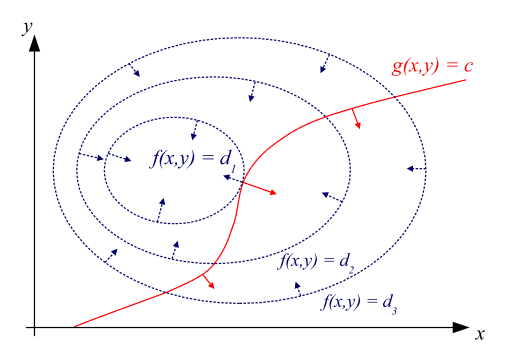
\includegraphics[width=0.95\linewidth]{img/LagrangeMultipliers2D.svg.png}
\end{center}

\end{frame}

%%%%%%%%%%%%%%%%%%%%%%%%%%%%%%%%%%%%%%%%%%%%%%%%%%%
\begin{frame}[fragile] \frametitle{}

For our problem we have:
\begin{align*}
L(a,\lambda) &= \sum_i a_i^2 + \lambda \cdot \left( 1 - \sum_i a_i x_i\right)
\end{align*}
Which gives:
\begin{align*}
\frac{\partial}{\partial a_k}  L(a,\lambda) &= 2 a_k - \lambda x_k \\
2 a_k - \lambda x_k &= 0 \\
a_k &= \frac{1}{2} \cdot \lambda \cdot x_k
\end{align*}

\end{frame}

%%%%%%%%%%%%%%%%%%%%%%%%%%%%%%%%%%%%%%%%%%%%%%%%%%%
\begin{frame}[fragile] \frametitle{}

The lambda derivative, which is just the constrain, shows the specific
value of $\lambda$ that we need:
\begin{align*}
\frac{\partial}{\partial \lambda}  L(a,\lambda) &= 1 - \sum_i a_i x_i \\
\sum_i a_i x_i &= 1
\end{align*}
\pause Plugging our previous version of $\lambda$:
\begin{align*}
\sum_i \frac{1}{2} \cdot \lambda \cdot x_i \cdot x_i &= 1 \\
\lambda \cdot \sum_i \frac{1}{2} \cdot x_i^2 &= 1 \\
\lambda &= \frac{2}{\sum_i x_i^2} \\
\end{align*}

\end{frame}

%%%%%%%%%%%%%%%%%%%%%%%%%%%%%%%%%%%%%%%%%%%%%%%%%%%
\begin{frame}[fragile] \frametitle{}

Finally, plugging this back in:
\begin{align*}
a_k &= \frac{1}{2} \cdot \lambda \cdot x_k \\
a_k &= \frac{x_k}{\sum_i x_i^2}
\end{align*}
And this gives:
\begin{align*}
\widehat{\beta}_{BLUE} &= \sum_i y_i \cdot \frac{x_i}{\sum_j x_j^2} \\
&= \widehat{\beta}_{MLE}
\end{align*}

\end{frame}

%%%%%%%%%%%%%%%%%%%%%%%%%%%%%%%%%%%%%%%%%%%%%%%%%%%
\begin{frame}[fragile] \frametitle{}

The MLE estimator has the following properties under our
assumptions:
\begin{itemize}
\item unbiased \pause
\item consistent as long as $\sum_i x_i^2$ diverges \pause
\item normally distributed \pause
\item is the BLUE estimator \pause
\item achieves the Cramér–Rao bound (problem set) \pause
\item has an analytic solution
\end{itemize}

\end{frame}


%%%%%%%%%%%%%%%%%%%%%%%%%%%%%%%%%%%%%%%%%%%%%%%%%%%
\begin{frame}[fragile] \frametitle{}

The more common formulation of simple linear models includes
an unknown intercept term $\alpha$. \pause The basic model is
then:
\begin{align*}
y_i &= \alpha + x_i\beta  + \epsilon_i, \quad i = 1, \ldots n.
\end{align*}

\end{frame}

%%%%%%%%%%%%%%%%%%%%%%%%%%%%%%%%%%%%%%%%%%%%%%%%%%%
\begin{frame}[fragile] \frametitle{}

The likelihood function for this revised model is almost the
same as before
\begin{eqnarray*}
\mathcal{L} (\beta, \sigma | x, y) &=& (2\pi\sigma^2)^{-n/2} \times
    exp \left\{ - \frac{1}{2\sigma^2} \cdot \sum_i {\color{solarized@orange} (y_i - \alpha - x_i\beta )^2} \right\} \\
\end{eqnarray*}
\pause Clearly, by the same logic the MLE is given by minimizing
the sum of squared residuals.

\end{frame}

%%%%%%%%%%%%%%%%%%%%%%%%%%%%%%%%%%%%%%%%%%%%%%%%%%%
\begin{frame}[fragile] \frametitle{}

Solving the least squares problem is only slightly more difficult
because now we have two parameters and need to use partial derivatives
to solve them. Otherwise the process is the same with a few more
terms floating around.

\end{frame}

%%%%%%%%%%%%%%%%%%%%%%%%%%%%%%%%%%%%%%%%%%%%%%%%%%%
\begin{frame}[fragile] \frametitle{}

The estimators in this case become:
\begin{align*}
\widehat{\beta} &= \frac{\sum_i (y_i - \bar{y})(x_i - \bar{x})}{\sum_i (x_i - \bar{x})^2} \\
\widehat{\alpha} &= \bar{y} - \widehat{\beta} \bar{x}
\end{align*}
Where $\bar{x} = n^{-1} \sum_i x_i$ and $\bar{y} = n^{-1} \sum_i y_i$. \pause

Notice what happens when both means are zero.

\end{frame}

%%%%%%%%%%%%%%%%%%%%%%%%%%%%%%%%%%%%%%%%%%%%%%%%%%%
\begin{frame}[fragile] \frametitle{}

All of these properties are maintained jointly for $(\widehat{\alpha}, \widehat{\beta})$
\begin{itemize}
\item unbiased
\item consistent as long as $\sum_i (x_i-\bar{x})^2$ diverges
\item normally distributed
\item is the BLUE estimator
\item achieves the Cramér–Rao bound
\item has an analytic solution
\end{itemize}

\end{frame}

%%%%%%%%%%%%%%%%%%%%%%%%%%%%%%%%%%%%%%%%%%%%%%%%%%%
\begin{frame}[fragile] \frametitle{}

\begin{flushright}
{\color{yaleblue}\sc\fontsize{1cm}{0cm}\selectfont Applications}
\end{flushright}

\end{frame}

%%%%%%%%%%%%%%%%%%%%%%%%%%%%%%%%%%%%%%%%%%%%%%%%%%%
\begin{frame}[fragile] \frametitle{}

\noindent
\begin{minipage}{0.35\textwidth}
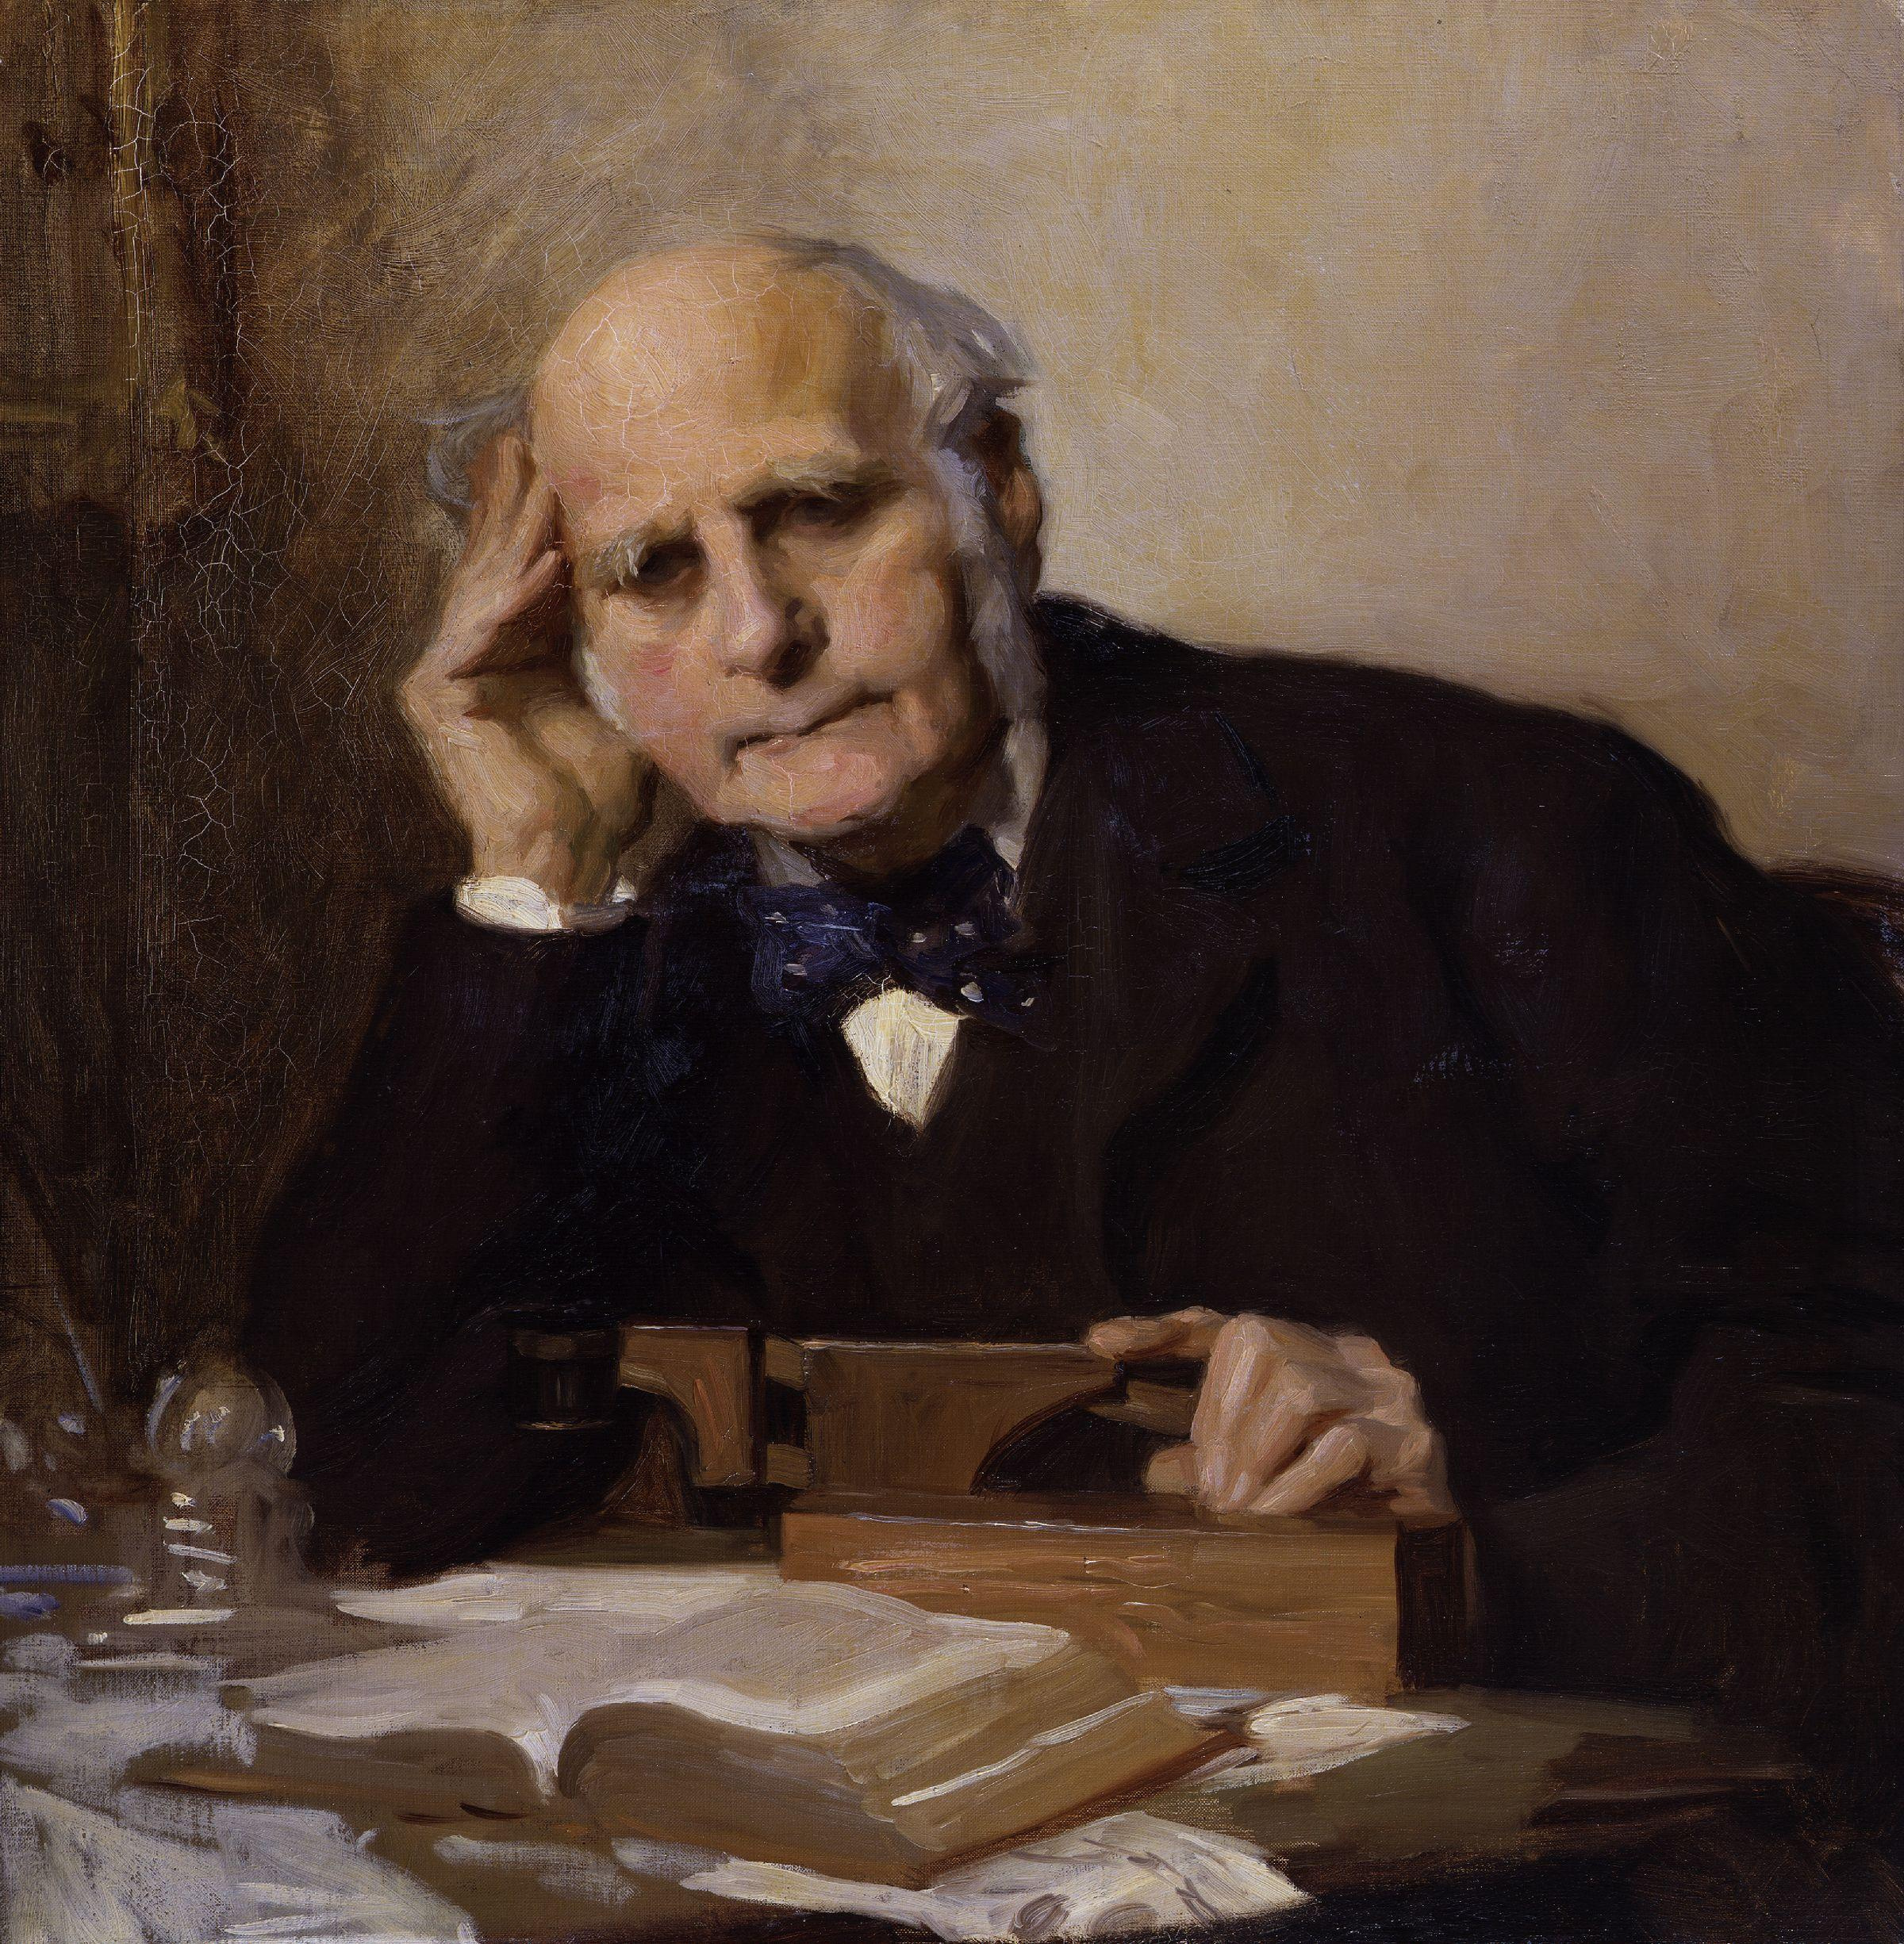
\includegraphics[width=0.75\linewidth]{img/Sir_Francis_Galton_by_Charles_Wellington_Furse.jpg}
\end{minipage}%%% to prevent a space
\begin{minipage}{0.65\textwidth}
Sir Francis Galton \& Regression \\
\begin{itemize}
\item `Co-relations and their measurement, chiefly from anthropometric data' (1888).
\item further ideas in {\it Natural Inheritance}
\begin{itemize}
\item sweet peas and regression to the mean
\item extinction of surnames (Galton–Watson stochastic processes)
\item `Good and Bad Temper in English Families'
\end{itemize}
\end{itemize}
\end{minipage}

\end{frame}


\end{document}













